% intro/intro.tex
% mainfile: ../perfbook.tex
% SPDX-License-Identifier: CC-BY-SA-3.0

\QuickQuizChapter{chp:Introduction}{简介}{qqzintro}
%
\Epigraph{如果并行编程真的那么难，为什么会有这么多并行程序？}{佚名}

并行编程已经获得了编程领域最难处理的问题之一这样的名声。
论文和教科书警告人们注意 \IX{deadlock}、\IX{livelock}、
\IXpl{race condition}、非确定性、
\IXaltr{Amdahl's-Law}{Amdahl's Law} 对扩展性的限制，
以及过高的实时延迟等种种危险。
这些危险确实真实存在；本书作者们已经积累了数不清的
% 2020:
%	30 for Paul E. McKenney
多年经验，连同由此产生的心理创伤、
白发和脱发。

然而，新技术在刚引入时总是难以使用，但随着时间的推移，终究会变得越来越容易。
例如，驾驶汽车曾经是一项罕见的技能，但在许多国家现在已经很普遍了。
这一巨大变化的产生基于两个基本原因：
\begin{enumerate*}[(1)]
\item 汽车变得更便宜、更容易获得，因此更多的人有机会学习驾驶，而且
\item 由于自动变速器、自动风门、自动启动器、大幅提高的可靠性以及许多其他技术改进，
汽车变得更容易操作。
\end{enumerate*}

对于许多其他技术来说也是如此，包括计算机。
如今编程已不再是一件困难的事情。
电子表格使大多数非程序员能够用计算机得到结果，
而在几十年前这需要专家才能胜任。
也许最具说服力的例子是网页浏览和内容创作，
自2000年代初以来，未经训练、未受过教育的人们
使用各种如今已司空见惯的社交网络工具就能轻松完成这些事情。
就在1968年，这样的内容创作还是一个超前的研究
项目~\cite{DouglasEngelbart1968}，
在当时被描述为``like a UFO landing on the White House lawn''~\cite{ScottGriffen2000}。
% http://www.ibiblio.org/pioneers/engelbart.html
% http://www.histech.rwth-aachen.de/www/quellen/engelbart/ahi62index.html

因此，如果你想说并行编程将一直保持目前许多人所认为的那么困难，
那么举证责任在你，请想一想在许多领域中有好几个世纪的反例。

\section{并行编程的历史困难}
\label{sec:intro:Historic Parallel Programming Difficulties}
%
\epigraph{不是记忆的力量，而恰恰是它的反面——遗忘的力量，才是我们存在的必要条件。}
	 {Sholem Asch}

正如本书标题所示，本书采取了一种不同的方法。
本书不是抱怨并行编程的困难，
而是认真分析并行编程困难的原因，
然后帮助读者克服这些困难。
我们将看到，这些困难在历史上主要分为以下几类：

\begin{enumerate}
\item	并行系统在历史上的高成本和相对稀缺性。
\item	典型研究人员和从业者缺乏并行系统的经验。
\item	公开可用的并行代码匮乏。
\item	缺乏被广泛理解的并行编程工程学科。
\item	即使在紧密耦合的 shared-memory 计算机中，通信相对于处理的高 \IX{overhead}。
\end{enumerate}

这些历史上的困难大多正在被克服。
首先，在过去几十年中，并行系统的成本已经从房价的数倍降低到一顿普通餐的价格，
这要归功于 \IXr{Moore's Law}~\cite{GordonMoore1965MooresLaw}。
早在1996年就有论文指出了多核 CPU 的优势~\cite{Olukotun96}。
IBM 在2000年将同步多线程（thread）技术引入其高端 \Power{} 系列，
并在2001年引入多核。
Intel 在2000年11月将超线程技术引入其商用 Pentium 产品线，
AMD 和 Intel 在2005年都推出了双核 CPU。
Sun 随后在2005年底推出了多核/多线程的 Niagara。
事实上，到2008年，想要找到一台单 CPU 的台式系统已经变得困难，
单核 CPU 被降级到上网本和嵌入式设备。
到2012年，连智能手机都开始配备多个 CPU 了。
到2020年，安全关键软件标准开始涉及并发问题。

其次，低成本且易于获得的多核系统的出现意味着，
曾经罕见的并行编程经验现在几乎所有研究人员和从业者都可以获得。
事实上，并行系统长期以来一直在学生和业余爱好者的预算范围之内。
因此，我们可以期待围绕并行系统的发明和创新会大幅增加，
而且日益增长的熟悉度将使并行编程飞入寻常百姓家。

第三，在20\textsuperscript{世纪}，大型高度并行的软件系统几乎总是作为严格保护的专有秘密。
让人欣慰的是，21\textsuperscript{世纪}恰恰相反，已经涌现出许多开源（因而公开可用的）
并行软件项目，包括 Linux 内核~\cite{Torvalds2.6kernel}、
数据库系统~\cite{PostgreSQL2008,MySQL2008}
和消息传递系统~\cite{OpenMPI2008,BOINC2008}。
本书将主要取材于 Linux 内核，但也会提供许多适用于用户态应用程序的内容。

第四，尽管1980年代和1990年代的大型并行编程项目几乎都是专有项目，
但这些项目已经孕育了开发者社区，其中的开发者深知生产级并行代码需要什么样的工程准则。
本书的一个主要目的就是展示这些工程准则。

不幸的是，第五个困难——通信相对于处理的高成本——在很大程度上仍然存在。
这一困难在新千年以来受到越来越多的关注。
然而，根据 \ppl{Stephen}{Hawking} 的说法，
有限的光速和物质的原子本性将限制
这一领域的进展~\cite{BryanGardiner2007,GordonMoore03a}。
幸运的是，这一困难自1980年代末就已经存在，
因此上述工程准则已经发展出实用且有效的应对策略。
此外，硬件设计者越来越意识到这些问题，
因此未来的硬件可能会对并行软件更加友好，
如 \cref{sec:cpu:Hardware Free Lunch?} 中所讨论的。

\QuickQuiz{
	拜托！！！
	几十年来，并行编程一直被认为极其困难。
	你似乎在暗示它并不那么难。
	你到底在玩什么把戏？
}\QuickQuizAnswer{
	如果你真的相信并行编程极其困难，
	那么你应该能随时回答这个问题：
	``为什么并行编程很难？''
	人们可以列出任何数量的原因，从 deadlock 到
	race condition 再到测试覆盖率，但真正的答案是
	{\em 它其实并没有那么难}。
	毕竟，如果并行编程真的如此可怕地困难，
	那么从 Apache 到 MySQL 再到 Linux 内核的大量开源项目
	是怎么掌握它的呢？

	一个更好的问题可能是：
	``为什么并行编程\emph{被认为}如此困难？''
	要找到答案，让我们回到1991年。
	Paul McKenney 正穿过停车场走向 Sequent 公司的
	基准测试中心，手里拿着六块双 80486 Sequent Symmetry CPU
	板，这时他突然意识到他手中所拿的东西价值是他刚买的
	房子的好几倍。\footnote{
		是的，这个突然的认识{\em 确实}让他走路小心多了。
		你为什么要问？}
	并行系统的高成本意味着并行编程仅限于少数特权阶层，
	他们的雇主要么是生产这种机器的厂商，
	要么有能力购买价值超过10万美元的机器——以1991年的美元计。

	相比之下，在2020年，Paul 发现自己正在一台六核 x86 笔记本电脑上
	敲下这些文字。
	与双 80486 CPU 板不同，这台笔记本还包含
	64\,GB 内存、1\,TB 固态硬盘、显示器、以太网、
	USB 端口、无线网络和蓝牙。
	而且这台笔记本的价格比那些双 80486 CPU 板中的任何一块
	都要低一个数量级以上，这还没有考虑通货膨胀因素。

	并行系统确实已经到来。
	它们不再是少数特权阶层的专属领域，而是几乎每个人都可以使用的东西。

	并行硬件早期受限的可用性才是并行编程被认为如此困难的
	\emph{真正}原因。
	毕竟，如果你无法接触到一台机器，即使是最简单的机器，
	学习编程也是相当困难的。
	既然罕见且昂贵的并行机器的时代已经基本过去，
	并行编程被认为令人崩溃般困难的时代也即将结束。\footnote{
		并行编程在某些方面确实比顺序编程更困难，
		例如并行验证更加困难。
		但不再是令人崩溃般的困难了。}
}\QuickQuizEnd

然而，即使并行编程没有通常宣传得那么难，
它也比顺序编程要麻烦不少。

\QuickQuiz{
	并行编程怎么可能像顺序编程一样\emph{简单}？
}\QuickQuizAnswer{
	这取决于编程环境。
	SQL~\cite{DIS9075SQL92} 是一个未被充分认识的成功案例，
	因为它允许完全不了解并行性的程序员
	让大型并行系统保持高效运转。
	随着并行计算机继续变得更便宜和更容易获得，
	我们可以期待更多这一主题的变体。
	例如，在科学和技术计算领域中的一个可能竞争者是 MATLAB*P，
	它试图自动并行化常见的矩阵运算。

	最后，在 Linux 和 UNIX 系统上，请考虑以下 shell 命令：

	\begin{VerbatimU}
	get_input | grep "interesting" | sort
	\end{VerbatimU}

	这个 shell 管道并行运行 \co{get_input}、\co{grep}
	和 \co{sort} 进程。
	看，这不难吧？

	简而言之，并行编程就像顺序编程一样简单——至少在那些向用户隐藏
	并行性的环境中是如此！
}\QuickQuizEnd

因此，思考并行编程的替代方案并非没有道理。
但是，如果不了解并行编程的目标，就不可能合理地思考并行编程的替代方案。
这一主题将在下一节中讨论。

\section{并行编程的目标}
\label{sec:intro:Parallel Programming Goals}
%
\epigraph{如果你不知道自己要去哪里，你最终会到达别的地方。}{Yogi Berra}

并行编程的三大目标（在顺序编程目标之上）如下：

\begin{enumerate}
\item	\IX{Performance}（性能）。
\item	\IX{Productivity}（生产力）。
\item	\IX{Generality}（通用性）。
\end{enumerate}

不幸的是，鉴于当前的技术水平，对于任何给定的并行程序，
最多只能实现这三个目标中的两个。
因此，这三个目标构成了\emph{并行编程的铁三角}，
一个过于乐观的希望经常在其上遭遇挫折的三角形。\footnote{
	感谢 Michael Wong 命名了铁三角。}

\QuickQuizSeries{%
\QuickQuizB{
	真的吗？？？
	那正确性、可维护性、鲁棒性等呢？
}\QuickQuizAnswerB{
	这些确实是重要的目标，但它们对顺序程序和并行程序同样重要。
	因此，尽管它们很重要，但不应出现在并行编程特有的列表中。
}\QuickQuizEndB
%
\QuickQuizM{
	如果正确性、可维护性和鲁棒性都不在列表中，
	为什么生产力和通用性在呢？
}\QuickQuizAnswerM{
	鉴于并行编程被认为比顺序编程难得多，
	生产力至关重要，因此不能被省略。
	此外，像 SQL 这样的高生产力并行编程环境服务于特定目的，
	因此通用性也必须加入列表。
}\QuickQuizEndM
%
\QuickQuizM{
	鉴于并行程序比顺序程序更难证明其正确性，
	正确性难道不应该\emph{真的}出现在列表中吗？
}\QuickQuizAnswerM{
	从工程角度来看，证明正确性的困难——无论是形式化的还是非形式化的——
	其重要性在于它对生产力这一主要目标的影响程度。
	因此，在正确性证明很重要的情况下，
	它被归入``生产力''的范畴之下。
}\QuickQuizEndM
%
\QuickQuizE{
	纯粹的乐趣呢？
}\QuickQuizAnswerE{
	乐趣也很重要，但除非你是业余爱好者，
	否则通常不会是\emph{主要}目标。
	另一方面，如果你\emph{确实}是业余爱好者，那就尽情享受吧！
}\QuickQuizEndE
}

以下各节将详细阐述这些目标。

\subsection{性能}
\label{sec:intro:Performance}

性能是大多数并行编程工作的首要目标。
毕竟，如果不需要考虑性能，何不让自己轻松一点，
直接编写顺序代码呢？
这样可能简单许多，而且你可能会更快地完成任务。

\QuickQuiz{
	难道没有并行编程不是为了性能的情况吗？
}\QuickQuizAnswer{
	当然有一些待解决的问题本质上就是并行的情况，
	例如蒙特卡罗方法和一些数值计算。
	然而即使在这些情况下，也会有一些管理并行性的额外工作。

	并行性有时也用于可靠性。
	举一个例子，三模冗余让三个系统并行运行并对结果进行投票。
	在极端情况下，三个系统会使用不同的算法和技术独立实现。
}\QuickQuizEnd

请注意，这里的``性能''是广义的，
包括例如 \IX{scalability}（每个 CPU 的性能）和 \IX{efficiency}（每瓦性能）。

\begin{figure}
\centering
\resizebox{3in}{!}{\includegraphics{SMPdesign/clockfreq}}
\caption{Intel CPU 的 MIPS/时钟频率趋势}
\label{fig:intro:Clock-Frequency Trend for Intel CPUs}
\end{figure}

话虽如此，对性能的关注焦点已经从硬件转向了并行软件。
这是因为，尽管 \IXr{Moore's Law}
仍然在晶体管密度方面持续有效，但它已经不再带来传统的单线程性能提升。
这可以从
\cref{fig:intro:Clock-Frequency Trend for Intel CPUs} 中看出，\footnote{
	此图显示了理论上能够每个时钟周期退休一条或多条指令的较新 CPU 的时钟频率，
	以及需要多个时钟周期执行最简单指令的较老 CPU 的 MIPS
	（每秒百万条指令，通常来自旧的 Dhrystone 基准测试）。
	在这两种度量之间切换的原因是，
	较新 CPU 每个时钟周期退休多条指令的能力通常受限于内存系统性能。
	此外，通常用于较老 CPU 的基准测试已经过时，
	而且很难在包含旧 CPU 的系统上运行较新的基准测试，
	部分原因是很难找到仍能工作的旧 CPU 实例。}
该图表明，编写单线程代码然后仅仅等待一两年让 CPU 赶上来，
可能不再是一个选项了。
鉴于所有主要制造商近年来都转向多核/多线程系统的趋势，
对于那些想要充分利用其系统全部性能的人来说，并行化是正确的方向。

\QuickQuiz{
	为什么不用 C 或 C++ 重写低效脚本语言编写的程序呢？
}\QuickQuizAnswer{
	如果有开发人员、预算和时间来进行这样的重写，
	并且重写的结果能在单个 CPU 上达到所需的性能水平，
	这可以是一个合理的方法。
}\QuickQuizEnd

即便如此，首要目标是性能而非可扩展性，
尤其是考虑到实现线性可扩展性的最简单方法就是
降低每个 CPU 的性能~\cite{LinusTorvalds2001a}。
假如有一个四 CPU 系统，你更喜欢哪个？
一个在单 CPU 上提供每秒100个事务但完全不可扩展的程序？
还是一个在单 CPU 上提供每秒10个事务但完美扩展的程序？
第一个程序似乎更好，尽管如果你碰巧有一个32 CPU 的系统，
答案可能会改变。

此外，即使你拥有多个 CPU，也不一定非要把它们全部用起来，
特别是考虑到多 CPU 系统近年来的价格不断下降。
理解这一点的关键是，并行编程本质上是一种性能优化，
而且只是众多潜在优化方法之一。
如果你的程序以目前的写法已经足够快了，那就没有理由去优化，
无论是通过并行化还是通过应用众多潜在的顺序优化方法。\footnote{
	当然，如果你是一个主要兴趣在于编写并行软件的业余爱好者，
	那么并行化你感兴趣的任何软件都是足够充分的理由。}
出于同样的道理，如果你想将并行性作为顺序程序的一种优化手段，
那么你需要将并行算法与最好的顺序算法进行比较。
这里需要注意，因为太多的出版物在分析并行算法的性能时
忽略了顺序算法的情况。

\subsection{生产力}
\label{sec:intro:Productivity}

\EQuickQuiz{
	为什么一直喋喋不休地谈论非技术问题？？？
	而且不是\emph{任何}非技术问题，偏偏是\emph{生产力}？
	谁在乎呢？
}\EQuickQuizAnswer{
	如果你是一个纯粹的业余爱好者，也许你不需要在乎。
	但即使是纯粹的业余爱好者，通常也会在意他们能做多少事、做多快。
	毕竟，最受欢迎的业余爱好者工具通常是最适合工作的工具，
	而``最适合''的定义中很重要的一部分就涉及生产力。
	如果有人付钱让你编写并行代码，他们很可能会非常关心你的生产力。
	如果付钱给你的人在乎某件事，你最好也至少给予一些关注！

	再说了，如果你\emph{真的}不在乎生产力，
	你应该手工做而不是用计算机！
}\EQuickQuizEnd

近几十年来，\IX{Productivity} 变得愈发重要。
要理解这一点，请想想早期计算机的价格高达数百万美元，
而当时工程师的薪水每年只有几千美元。
假如为这样一台机器配上一个十人工程师团队，
即使他们只能将性能提高10\pct，这也相当于付出薪水的很多倍了。

这样的一台机器是 CSIRAC，它是现存最古老的完整全电子存储程序计算机，
于1949年投入运行~\cite{CSIRACMuseumVictoria,CSIRACUniversityMelbourne}。
由于这台机器建造于晶体管时代之前，它由2,000个真空管构成，
时钟频率为1\,kHz，功耗30\,kW，重量超过三公吨。
鉴于这台机器只有768个字的 RAM，可以说它不会遭受
经常困扰当今大型软件项目的生产力问题。

如今，要购买一台计算能力如此之低的机器已经相当困难了。
也许最接近的等价物是以经典的 Z80~\cite{z80Wikipedia} 为代表的8位嵌入式微处理器，
但即使是旧的 Z80 的 CPU 时钟频率也比 CSIRAC 快1,000倍以上。
Z80 CPU 有8,500个晶体管，在2008年以1,000个单位的数量购买时
每个不到 \$2 美元。
与 CSIRAC 形成鲜明对比的是，Z80 的软件开发成本绝非微不足道。

\begin{figure}
\centering
\resizebox{3in}{!}{\includegraphics{SMPdesign/mipsperbuck}}
\caption{Intel CPU 每个裸片的 MIPS}
\label{fig:intro:MIPS per Die for Intel CPUs}
\end{figure}

CSIRAC 和 Z80 是一个长期趋势中的两个点，这可以从
\cref{fig:intro:MIPS per Die for Intel CPUs} 中看出。
该图绘制了过去四十年中每个裸片计算能力的近似值，
显示了四十年内令人印象深刻的六个数量级的增长。
请注意，多核 CPU 的出现使这一增长得以继续快速推进，
尽管在2003年遭遇了时钟频率墙，但每个裸片支持超过50个硬件线程功不可没。

硬件成本快速下降的一个不可避免的后果是，
软件生产力变得越来越重要。
仅仅高效地使用硬件已经不够了，高效地利用软件开发人员已经变得同样重要。
对于顺序硬件来说，这早已如此，
但并行硬件只是在最近才变成低成本的商品。
因此，在创建并行软件时，高生产力只是在最近才变得至关重要。

\QuickQuiz{
	既然并行系统已经变得如此便宜，怎么还有人能付得起程序员来编程呢？
}\QuickQuizAnswer{
	这个问题有多个答案：
	\begin{enumerate}
	\item	对于一个由并行机器组成的大型计算集群，
		集群的总成本很容易证明大量开发人员投入的合理性，
		因为开发成本可以分摊到大量机器上。
	\item	被数千万用户使用的流行软件可以轻松证明大量
		开发人员投入的合理性，因为开发成本可以分摊到
		数千万用户上。
		请注意这包括内核和系统库等。
	\item	如果低成本并行机器控制着一台贵重设备的运行，
		那么这台设备的成本可能很容易证明大量
		开发人员投入的合理性。
	\item	如果低成本并行机器的软件产生了极有价值的结果
		（例如节能），那么这一有价值的结果同样可以
		证明大量开发成本的合理性。
	\item	安全关键系统保护生命，这显然可以证明
		非常大的开发人员投入的合理性。
	\item	业余爱好者和研究人员可能追求的是知识、
		经验、乐趣或荣誉。
	\end{enumerate}
	因此，并非硬件成本的降低使软件变得毫无价值，
	而是不再可能将软件开发成本``隐藏''在硬件成本中，
	除非有极其大量的硬件。
}\QuickQuizEnd

也许曾经并行软件的唯一目的是性能。
然而现在，生产力正在受到越来越多的关注。

\subsection{通用性}
\label{sec:intro:Generality}

降低并行软件高开发成本的一种方法是
追求最大化的 \IX{generality}。
在其他条件相同的情况下，更通用的软件能获得更多的用户，
从而将开发成本分摊到更多用户身上。
事实上，这种经济力量解释了对可移植性的疯狂关注，
可移植性可以被视为通用性的一个重要特例。\footnote{
	感谢 Michael Wong 指出了这一点。}

不幸的是，通用性通常以牺牲性能、生产力或两者为代价。
例如，可移植性通常通过适配层来实现，
这不可避免地会带来性能损失。
为了更一般性地理解这一点，请考虑以下流行的并行编程环境：

\begin{description}
\item[C/C++ ``Locking Plus Threads''：] 这一类别包括
	POSIX Threads (pthreads)~\cite{OpenGroup1997pthreads}、
	Windows Threads 以及众多操作系统内核环境，
	提供出色的性能（至少在单个 SMP 系统的范围内），
	同时也提供良好的通用性。
	可惜生产力相对较低。
\item[Java：] 这种通用且本质上支持多线程的编程环境
	被广泛认为比 C 或 C++ 提供高得多的生产力，
	这归功于自动垃圾收集器和丰富的类库集。
	然而，它的性能虽然在2000年代初大幅提高，但仍落后于 C 和 C++。
\item[MPI：] 这种 Message Passing Interface~\cite{MPIForum2008}
	驱动着世界上最大的科学和技术计算集群，
	提供无与伦比的性能和可扩展性。
	理论上它是通用的，但主要用于科学和技术计算。
	许多人认为它的生产力甚至低于 C/C++ ``locking plus threads'' 环境。
\item[OpenMP：] 这组编译器指令可用于并行化循环。
	因此它非常专注于这项任务，而这种专注性通常限制了它的性能。
	然而，它比 MPI 或 C/C++ ``locking plus threads'' 容易使用得多。
\item[SQL：] Structured Query Language~\cite{DIS9075SQL92}
	专用于关系数据库查询。
	然而，根据事务处理性能委员会（TPC）基准测试结果~\cite{TPC}
	的衡量，它的性能相当好。
	生产力非常出色；事实上，这种并行编程环境使人们能够充分利用
	大型并行系统，即使他们对并行编程概念知之甚少或完全不了解。
\end{description}

\QuickQuiz{
	SQL？？？
	那是古老的历史了。
	在2020年代，如果你真的想充分利用大型并行系统，
	为什么不使用机器学习呢？
}\QuickQuizAnswer{
	机器学习确实能让许多大型并行系统保持忙碌！
	然而，这是否构成对这些系统的\emph{良好}利用，
	陪审团仍在审议之中。
}\QuickQuizEnd

\begin{figure}
\centering
\resizebox{2.5in}{!}{\includegraphics{intro/PPGrelation}}
\caption{软件层次与性能、生产力和通用性}
\label{fig:intro:Software Layers and Performance; Productivity; and Generality}
\end{figure}

并行编程环境的涅盘——一个同时提供世界级性能、
生产力和通用性的环境——目前还不存在。
在这样一个涅盘出现之前，我们有必要在性能、生产力和通用性之间
进行工程权衡。
其中一种权衡如
\cref{fig:intro:Software Layers and Performance; Productivity; and Generality}
中所示的绿色``铁三角''\footnote{
	感谢 Michael Wong 创造了``铁三角''一词。}所描绘的那样，
该图说明了这样一个事实：越往系统栈上层，生产力变得越来越重要；
而越往下层，性能和通用性变得越来越重要。
一方面，下层产生的巨大开发成本必须分摊到同样巨大数量的用户上
（因此通用性很重要），而且在底层损失的性能
无法在更高层轻松恢复。
另一方面，在栈的上层，对于一个给定的特定应用可能只有很少的用户，
在这种情况下生产力问题至关重要。
这解释了栈上层趋向``臃肿软件''的倾向：
采用额外的硬件通常比额外的开发人员更划算。
本书面向在栈底层工作的开发人员，主要关注性能和通用性。

\begin{figure}
\centering
\resizebox{3in}{!}{\includegraphics{intro/Generality}}
\caption{生产力与通用性之间的权衡}
\label{fig:intro:Tradeoff Between Productivity and Generality}
\end{figure}

不得不承认，生产力和通用性之间的权衡在许多领域已经存在了几个世纪。
举一个例子，钉枪在打钉子方面远比锤子高效，
但与钉枪不同，锤子除了打钉子外还能做许多其他事情。
因此，在并行计算领域看到类似的权衡也就不足为奇了。
这种权衡示意性地显示在
\cref{fig:intro:Tradeoff Between Productivity and Generality} 中。
这里，用户~1、2、3和~4有他们需要计算机帮助完成的特定工作。
对于给定用户来说，最高效的语言或环境是
直接完成该用户工作的那个，无需任何编程、配置或其他设置。

\QuickQuiz{
	这是一个荒谬的、不可能实现的理想！
	为什么不专注于实际中可以实现的东西呢？
}\QuickQuizAnswer{
	这是完全可以实现的。
	手机就是一台可以用来打电话和收发短信的计算机，
	而终端用户几乎不需要进行任何编程或配置。

	乍一看这似乎是一个微不足道的例子，
	但如果你仔细考虑就会发现它既简单又深刻。
	当我们愿意牺牲通用性时，我们可以在生产力方面取得
	真正惊人的提升。
	因此，那些沉迷于过度通用性的人将无法将生产力标准
	设定得足够高以在软件栈顶部获得成功。
	这一事实甚至有自己的缩写：
	YAGNI，即``You Ain't Gonna Need It''（你不会需要它的）。
}\QuickQuizEnd

不幸的是，在用户~1的工作上表现最优的系统
不太可能在用户~2的工作上表现很好。
换句话说，最高效的语言和环境是领域特定的，
因此根据定义缺乏通用性。

另一种选择是将给定的编程语言或环境定制为
适合硬件系统（例如低级语言如汇编、C、C++ 或 Java）
或某种抽象（例如 Haskell、Prolog 或 Snobol），
如 \cref{fig:intro:Tradeoff Between Productivity and Generality}
中心附近的圆形区域所示。
这些语言可以被认为是通用的，因为它们对用户~1、2、3和~4
的工作同样不太适合。
也就是说，与领域特定的语言和环境相比，
它们的通用性是以牺牲生产力为代价获得的。
更糟糕的是，针对给定抽象定制的语言
很可能会遭受性能和可扩展性问题，
除非并且直到它能被高效地映射到真实硬件上。

难道就没有办法逃脱铁三角中性能、生产力和通用性这三个相互冲突的目标吗？

事实证明，通常是有办法逃脱的，例如，
使用下一节讨论的并行编程替代方案。
毕竟，并行编程可以非常有趣，但它并不总是最合适的工具。

\section{并行编程的替代方案}
\label{sec:intro:Alternatives to Parallel Programming}
%
\epigraph{当经验已经指明道路时，实验就是愚蠢的。}
	 {Roger M. Babson}

在考虑并行编程的替代方案之前，
你必须首先想清楚你到底期望并行性为你做什么。
如 \cref{sec:intro:Parallel Programming Goals} 中所述，
并行编程的主要目标是性能、生产力和通用性。
由于本书面向在软件栈底部处理性能关键代码的开发人员，
本节的其余部分主要关注性能提升。

重要的是要记住，并行化只是提高性能的方法之一。
其他众所周知的方法包括以下几种，大致按难度递增排列：

\begin{enumerate}
\item	运行顺序应用程序的多个实例。
\item	让应用程序使用现有的并行软件。
\item	优化顺序应用程序。
\end{enumerate}

这些方法将在以下各节中介绍。

\subsection{运行顺序应用程序的多个实例}
\label{sec:intro:Multiple Instances of a Sequential Application}

通过运行顺序应用程序的多个实例，可以让你在不实际进行并行编程的情况下
利用并行性。
根据应用程序的结构，有很多方法可以实现这一点。

如果你的程序正在分析大量不同的场景，
或者正在分析大量独立的数据集，一个简单有效的方法是
创建一个执行单次分析的顺序程序，
然后使用众多脚本环境中的任何一个（例如 \co{bash} shell）
来并行运行该顺序程序的多个实例。
在某些情况下，这种方法可以轻松扩展到机器集群。

这种方法可能看起来像是作弊，事实上有些人贬低这样的程序为
``\IX{embarrassingly parallel}''（令人尴尬的并行）。
而且实际上，这种方法确实有一些潜在的缺点，
包括增加内存消耗、浪费 CPU 周期重新计算公共中间结果以及增加数据复制。
然而，它通常极其高效，以很少甚至没有额外的努力
就能获得极高的性能增益。

\subsection{使用现有的并行软件}
\label{sec:intro:Use Existing Parallel Software}

能够提供单线程编程环境的并行软件已不再缺乏，包括关系
数据库~\cite{Date82}、Web 应用服务器和 map-reduce 环境。
例如，一种常见的设计是为每个用户提供一个单独的进程，
每个进程根据用户查询生成 SQL 语句，
然后在一个公共关系数据库上并发执行。
每个用户的程序只需负责用户界面，
而关系数据库则负责处理所有围绕并行性和持久性的困难问题。

此外，并行库函数的数量也在不断增长，特别是用于数值计算的库。
更好的是，一些库利用了专用硬件，
如向量单元和通用图形处理单元（GPGPU）。

采用这种方法通常会牺牲一些性能，至少与仔细手工编码完全并行的
应用程序相比是这样。
然而，这种牺牲通常可以通过开发工作量的巨大减少来充分回报。

\QuickQuiz{
	等一下！
	这种方法不就是简单地将开发工作从你转移到
	编写你正在使用的现有并行软件的人身上吗？
}\QuickQuizAnswer{
	没错！
	这正是使用现有软件的全部意义。
	一个团队的工作可以被许多其他团队使用，
	与所有团队都不必要地重新发明轮子相比，
	整体工作量大幅减少。
}\QuickQuizEnd

\subsection{性能优化}
\label{sec:intro:Performance Optimization}

直到2000年代初，CPU 时钟频率每18个月翻一番。
在这样的背景下，增加新功能的重要性通常远大于仔细优化性能。
现在 \IXr{Moore's Law} ``只是''增加晶体管密度而不是
同时增加晶体管密度和每个晶体管的性能，
也许是时候重新思考性能优化的重要性了。
毕竟，新一代硬件不再带来显著的单线程性能提升。
此外，许多性能优化也可以节约能源。

从这个角度来看，并行编程只是另一种性能优化，
尽管随着并行系统变得更便宜、更容易获得，它正变得越来越有吸引力。
然而，明智的做法是记住，并行化所能获得的加速大约限于 CPU 的数量
（但请参阅 \cref{sec:SMPdesign:Beyond Partitioning}
了解一个有趣的例外）。
相比之下，传统单线程软件优化所能获得的加速可能大得多。
例如，将一个长链表替换为哈希表（hash table）或搜索树可以将性能提高好几个数量级。
这种高度优化的单线程程序可能比未优化的并行程序运行得快得多，
使得并行化变得不必要。
当然，一个高度优化的并行程序会更好，
只是需要额外的开发工作。

此外，不同的程序会有不同的性能瓶颈。
例如，如果你的程序大部分时间都在等待磁盘的数据，
使用多个 CPU 可能只是增加了等待磁盘的浪费时间。
事实上，如果程序正在从旋转磁盘上顺序排列的单个大文件中读取数据，
并行化你的程序很可能会由于额外的寻道开销而使其变慢很多。
你应该改为优化数据布局，使文件可以更小（因此读取更快），
将文件分成可以从不同驱动器并行访问的块，
将频繁访问的数据缓存在主存中，
或者如果可能的话，减少必须读取的数据量。

\QuickQuiz{
	还有哪些瓶颈可能阻止额外的 CPU 提供额外的性能？
}\QuickQuizAnswer{
	有许多潜在的瓶颈：
	\begin{enumerate}
	\item	主存。
		如果单个 thread 消耗了所有可用内存，
		额外的 thread 只会疯狂地进行页面交换。
	\item	Cache。
		如果单个 thread 的 cache 占用完全填满了任何共享 CPU cache，
		那么添加更多 thread 只会使受影响的 cache 剧烈抖动，
		正如 \cref{chp:Data Structures} 中将要看到的。
	\item	内存带宽。
		如果单个 thread 消耗了所有可用的内存带宽，
		额外的 thread 只会导致系统互连上的额外排队。
	\item	I/O 带宽。
		如果单个 thread 是 I/O 受限的，
		添加更多 thread 只会导致它们都在排队
		等待受影响的 I/O 资源。
	\end{enumerate}

	特定的硬件系统可能有许多额外的瓶颈。
	事实上，在多个 CPU 或 thread 之间共享的
	每个资源都是潜在的瓶颈。
}\QuickQuizEnd

并行化可以是一种强大的优化技术，但它并不是唯一的优化技术，
也并非适合所有情况。
当然，你的程序越容易并行化，并行化作为一种优化就越有吸引力。
并行化号称非常困难，
这就引出了一个问题：``究竟是什么使并行编程如此困难？''

\section{是什么使并行编程如此困难？}
\label{sec:intro:What Makes Parallel Programming Hard?}
%
\epigraph{真正的困难可以被克服；只有想象中的困难才是不可战胜的。}{Theodore N.~Vail}

\OriginallyPublished{sec:intro:What Makes Parallel Programming Hard?}{What Makes Parallel Programming Hard?}{a Portland State University Technical Report}{PaulEMcKenney2009ProgrammingHard}

需要注意的是，并行编程的困难既有人为因素的原因，
也有并行编程本身技术属性的原因。
我们确实需要人来告诉计算机该做什么，
换句话说，就是编程。
但并行编程需要双向交互：人还需要从计算机处得到
程序性能和可扩展性的反馈。
简而言之，人类通过编写程序告诉计算机该做什么，
而计算机通过产生的性能和可扩展性来评价这个程序。
因此，采用抽象或数学分析将极大地限制实用性。

在工业革命中，人与机器之间的接口通过人因研究来评估，
即当时所谓的工时与动作研究。
虽然有一些人因研究检验了并行编程
~\cite{RyanEccles2005HPCSNovice,RyanEccles2006HPCSNoviceNeeds,
LorinHochstein2005SC,DuaneSzafron1994PEMPDS}，但这些研究
关注面过窄，因此无法得出任何一般性的结论。
此外，鉴于程序员生产力的正常范围跨越一个数量级以上，
期望一个可负担的研究能够检测到（比如说）10\pct\ 的生产力差异
是不现实的。
虽然此类研究\emph{能够}可靠检测到的多个数量级差异确实极其有价值，
但最令人印象深刻的改进往往是基于一长串10\pct 的改进。

因此，我们必须采取不同的方法。

\begin{figure}
\centering
\resizebox{3in}{!}{\includegraphics{intro/FourTaskCategories}}
\caption{并行程序员所需的任务类别}
\label{fig:intro:Categories of Tasks Required of Parallel Programmers}
\end{figure}

一种这样的方法是仔细考虑并行程序员必须承担的、
顺序程序员不需要承担的任务。
然后我们可以评估给定的编程语言或环境在多大程度上
帮助开发人员完成这些任务。
这些任务分为
\cref{fig:intro:Categories of Tasks Required of Parallel Programmers}
中所示的四个类别，每个类别将在以下各节中介绍。

\subsection{工作划分}
\label{sec:intro:Work Partitioning}

工作划分对于并行执行是绝对必要的：
如果只有一个不可划分的工作项，那么它最多只能由一个 CPU 在同一时间执行，
这根据定义就是顺序执行。
然而，划分工作需要非常小心。
例如，不均匀的划分可能导致在小分区完成后变成
顺序执行~\cite{GeneAmdahl1967AmdahlsLaw}。
在不那么极端的情况下，可以使用负载均衡来充分利用
可用硬件并恢复性能和可扩展性。

虽然划分可以大大提高性能和可扩展性，
但它也会增加复杂性。
例如，划分可能使全局错误和事件的处理变得复杂：
并行程序可能需要执行非平凡的同步操作
才能安全地处理此类全局事件。
概括地说，每个分区都需要某种形式的通信：
毕竟，如果一个给定的 thread 完全不进行通信，
那么它不执行也不会产生任何影响。
然而，由于通信会产生开销，不仔细地选择划分方式
可能导致严重的性能下降。

此外，并发 thread 的数量通常必须加以控制，
因为每个这样的 thread 都会占用公共资源，例如 CPU cache 中的空间。
如果允许太多 thread 并发执行，CPU cache 将溢出，
导致高 cache miss 率，进而降低性能。
反过来，通常需要大量 thread 来重叠计算和 I/O
以充分利用 I/O 设备。

\QuickQuiz{
	除了 CPU cache 容量之外，还有什么可能需要限制
	并发 thread 的数量？
}\QuickQuizAnswer{
	有许多对 thread 数量的潜在限制：
	\begin{enumerate}
	\item	主存。
		每个 thread 消耗一些内存（至少是它的栈），
		因此过多的 thread 可能耗尽内存，
		导致过度的页面交换或内存分配失败。
	\item	I/O 带宽。
		如果每个 thread 发起一定量的大容量存储 I/O
		或网络流量，过多的 thread 可能导致过度的
		I/O 排队延迟，同样降低性能。
		某些网络协议如果有太多 thread 导致
		网络事件无法及时响应，可能会
		超时或出现其他故障。
	\item	同步开销。
		对于许多同步协议，过多的 thread
		可能导致过度的自旋、阻塞或回滚，从而降低性能。
	\end{enumerate}

	特定的应用程序和平台可能有许多额外的限制因素。
}\QuickQuizEnd

最后，允许 thread 并发执行会大大增加程序的状态空间，
让程序难以理解和调试，从而降低生产力。
在其他条件相同的情况下，状态空间更小且结构更规则的程序
更容易理解，不过这只是与人相关的因素，
并非技术或数学上的因素。
好的并行设计可能拥有极大的状态空间，
但由于其规则的结构而并不难以理解；
而糟糕的设计即使状态空间相对较小也可能深奥难懂。
最好的设计利用 embarrassingly parallel，
或将问题转化为具有 embarrassingly parallel 解决方案的问题。
在任一情况下，``embarrassingly parallel'' 实际上是
一种令人尴尬的财富。
当前的技术水平枚举了好的设计；
对状态空间大小和结构做更一般性的判断还需要更多的工作。

\subsection{并行访问控制}
\label{sec:Parallel Access Control}

给定一个单线程顺序程序，该单个 thread 对程序的所有资源具有完全访问权限。
这些资源通常是内存中的数据结构，但也可以是 CPU、内存（包括 cache）、
I/O 设备、计算加速器、文件和许多其他东西。

第一个并行访问控制问题是，对给定资源的访问形式是否取决于该资源的位置。
例如，在许多消息传递环境中，局部变量的访问通过表达式和赋值进行，
而远程变量的访问使用完全不同的语法，通常涉及消息传递。
POSIX Threads 环境~\cite{OpenGroup1997pthreads}、
Structured Query Language (SQL)~\cite{DIS9075SQL92} 以及
分区全局地址空间 (PGAS) 环境
如 Universal Parallel C (UPC)~\cite{ElGhazawi2003UPC,UPCConsortium2013}
提供隐式访问，
而 Message Passing Interface (MPI)~\cite{MPIForum2008} 提供
显式访问，因为访问远程数据需要显式的消息传递。

另一个并行访问控制问题是 thread 如何协调对资源的访问。
这种协调是通过各种并行语言和环境提供的
大量同步机制来完成的，
包括消息传递、locking、事务、
引用计数（reference counting）、显式定时、共享 atomic 变量和数据所有权（data ownership）。
许多传统的并行编程关注点如 \IX{deadlock}、
\IX{livelock} 和事务回滚都源于这种协调。
这个框架可以扩展为包含这些同步机制的比较，
例如 locking 与 transactional memory~\cite{McKenney2007PLOSTM}
之间的比较，但这种扩展超出了本节的范围。
（参见 \cref{sec:future:Transactional Memory,%
sec:future:Hardware Transactional Memory}
了解关于 transactional memory 的更多信息。）

\QuickQuiz{
	``显式定时''到底是什么？？？
}\QuickQuizAnswer{
	每个 thread 在约定的时间槽内被授予对一组资源的访问权限。
	例如，一个有八个 thread 的并行程序可以组织为
	八毫秒的时间间隔，使得第一个 thread 在每个间隔的
	第一个毫秒内被授予访问权限，第二个 thread 在第二个毫秒，
	以此类推。
	这种方法显然需要精确同步的时钟和对执行时间的仔细控制，
	因此应该谨慎使用。

	事实上，在硬实时环境之外，你几乎肯定应该使用其他方法。
	然而，显式定时仍然值得一提，因为当你需要它时
	它总是在那里。
}\QuickQuizEnd

\subsection{资源划分与复制}
\label{sec:Resource Partitioning and Replication}

最有效的并行算法和系统非常善于利用资源并行性，
因此通常明智的做法是从划分写密集型资源和
复制频繁访问的读为主资源开始并行化。
讨论的资源最常见的是数据，它可能在计算机系统、
大容量存储设备、\IXplr{NUMA node}、CPU 核心（或裸片或硬件线程）、
页面、cache line、同步原语实例或代码临界区之间进行划分。
例如，在 locking 原语上的划分被称为
``\IXh{data}{locking}''~\cite{Beck85}。

资源划分通常取决于应用程序。
例如，数值应用程序经常按行、列或子矩阵划分矩阵，
而商业应用程序经常划分写密集型数据结构并复制读为主的数据结构。
因此，商业应用程序可能将给定客户的数据分配给
大型集群中特定的几台计算机。
应用程序可能静态划分数据，或随时间动态改变划分方式。

\begin{figure}
\centering
\resizebox{3in}{!}{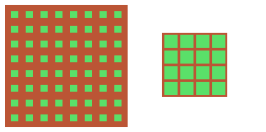
\includegraphics{intro/coarsen}}
\caption{粗粒度划分减少同步开销}
\label{fig:intro:Coarse Partitioning Reduces Synchronization Overhead}
\end{figure}

资源划分极其有效，但对于复杂的多链接数据结构
来说可能非常具有挑战性。
作为一个粗略的经验法则，你应该保持满足可扩展性目标所需的
最少分区数量，使每个分区尽可能大。

这种方法的目标是减少同步开销所消耗的时间比例，
如 \cref{fig:intro:Coarse Partitioning Reduces Synchronization Overhead}
所示，其中绿色区域代表有用的工作，深色区域代表同步开销。
当然，右边较粗的同步只有16个分区，
而左边有64个分区，然而，
很可能额外的同步开销将压过使用64个 CPU 而非16个
所可能带来的任何性能收益。

\QuickQuiz{
	这听起来像是一个困难的权衡。
	开发人员到底应该如何解决它？？？
}\QuickQuizAnswer{
	在可用硬件上测试不同的划分方案通常是最好的方法。
	但不要忘记用复制替代划分的可能性，
	这将在 \cref{sec:datastruct:Read-Mostly Data Structures} 中展示。
}\QuickQuizEnd

\subsection{与硬件交互}
\label{sec:Interacting With Hardware}

与硬件的交互通常是操作系统、编译器、库或其他软件环境基础设施的领域。
然而，使用新颖硬件特性和组件的开发人员通常需要直接与此类硬件打交道。
此外，当要从给定系统中挤出最后一滴性能时，可能需要直接访问硬件。
在这种情况下，开发人员可能需要根据目标硬件的 cache 几何结构、
系统拓扑或互连协议来定制或配置应用程序。

在某些情况下，硬件可以被视为一种资源，
可以进行划分或访问控制，如前几节所述。

\subsection{组合能力}
\label{sec:Composite Capabilities}

\begin{figure}
\centering
\resizebox{3in}{!}{\includegraphics{intro/FourTaskOrder}}
\caption{并行编程任务的顺序}
\label{fig:intro:Ordering of Parallel-Programming Tasks}
\end{figure}

虽然这四种能力是基本的，
但良好的工程实践会组合使用这些能力。
例如，数据并行方法首先划分数据以最小化分区间通信的需求，
相应地划分代码，
最后映射数据分区和 thread 以最大化吞吐量
同时最小化 thread 间通信，
如 \cref{fig:intro:Ordering of Parallel-Programming Tasks} 所示。
然后开发人员每次只需单独考虑一个分区，
显著减少了相关状态空间的大小，进而提高了生产力。
即使有些问题是不可划分的，
巧妙地将其转换为可以划分的形式有时可以大大提高
性能和可扩展性~\cite{PanagiotisMetaxas1999PDCS}。

\subsection{现有的顺序设计}
\label{sec:intro:Existing Sequential Designs}

现有的顺序程序设计可能是一个限制因素，
特别是在将系统适配为多核系统运行时，
面临着进行最小更改的巨大压力。
例如，考虑以下可能在顺序代码中使用的哈希表 API：

\begin{VerbatimU}
int hash_add(struct htab *htp);
int hash_del(int key);
struct htab *hash_lookup(int key);
\end{VerbatimU}

这里，\co{hash_add()} 和 \co{hash_del()} 都返回操作完成后
哈希表中元素的精确数量，或者如果操作因重复键或不存在的键而失败，
则分别返回 \co{-1}。
\co{hash_lookup()} 函数接受一个键并返回指向
相应元素的指针，如果没有这样的元素则返回 \co{NULL}。

这个 API 的问题在于 \co{hash_add()} 和 \co{hash_del()} 返回的精确计数。
虽然在顺序代码中维护和返回这些计数几乎是免费的，
但在多核系统上这样做可能极其昂贵并且会限制可扩展性，
如 \cref{chp:Counting} 中所讨论的。
修复这个并行编程问题的一种方法是让这些函数
改为返回近似计数（同样如 \cref{chp:Counting} 中所讨论的），
或者让它们对元素数量保持沉默，
如 \cref{sec:datastruct:Partitionable Data Structures} 中所讨论的。

当然还有许多其他在顺序代码中工作良好
但在并发代码中不行的设计模式。
然而，这个例子应该能让你对要注意什么有一个好的认识。

\subsection{语言和环境如何协助完成这些任务？}
\label{sec:intro:How Do Languages and Environments Assist With These Tasks?}

虽然许多环境要求开发人员手动处理这些任务，
但有一些历史悠久的环境可以带来显著的自动化。
这些环境的典范是 SQL，它的许多实现自动并行化
单个大型查询，还自动并发执行独立的查询和更新。

这四类任务必须在所有并行程序中执行，
但这当然并不一定意味着开发人员必须手动执行这些任务。
随着并行系统持续变得更便宜、更容易获得，
我们可以期待看到这四项任务的自动化程度不断提高。

\QuickQuiz{
	并行编程还有其他障碍吗？
}\QuickQuizAnswer{
	并行编程还有许多其他潜在障碍。
	以下是其中一些：
	\begin{enumerate}
	\item	给定项目的唯一已知算法可能
		本质上是顺序的。
		在这种情况下，要么避免并行编程
		（没有法律规定你的项目\emph{必须}并行运行），
		要么发明一种新的并行算法。
	\item	项目允许共享同一地址空间的纯二进制插件，
		使得没有任何一个开发人员能访问
		项目的全部源代码。
		因为许多并行 bug，包括 deadlock，
		在本质上是全局性的，这样的纯二进制插件
		对当前的软件开发方法论构成严峻挑战。
		这种情况可能会改变，但目前，共享给定地址空间的
		所有并行代码开发人员都需要能够看到
		在该地址空间中运行的\emph{所有}代码。
	\item	项目包含大量使用的、
		在设计时未考虑并行性的 API~\cite{HagitAttiya2011LawsOfOrder,Clements:2013:SCR:2517349.2522712}。
		System V 消息队列 API 的一些更华丽的特性就是一个典型例子。
		当然，如果你的项目已经存在了几十年，
		且其开发人员无法获得并行硬件，
		那么它无疑至少有其份额的此类 API。
	\item	项目在实现时未考虑并行性。
		鉴于有大量技术在顺序环境中运行得非常好
		但在并行环境中惨遭失败，
		如果你的项目在其大部分生命周期中
		只在顺序硬件上运行，
		那么你的项目无疑至少有其份额的对并行不友好的代码。
	\item	项目在实现时未遵循良好的软件开发实践。
		残酷的事实是，shared-memory 并行环境
		通常比顺序环境对草率的开发实践
		宽容得多。
		在尝试并行化之前清理现有的设计和代码
		可能对你很有好处。
	\item	最初在你的项目上做开发的人已经离开了，
		而留下的人虽然能够很好地维护项目或添加小功能，
		但无法进行``大手术''式的更改。
		在这种情况下，除非你能找到一种
		非常简单的方法来并行化你的项目，
		否则你最好让它保持顺序。
		话虽如此，有一些简单的方法你可以用来
		并行化你的项目，包括运行它的多个实例、
		使用某个大量使用的库函数的并行实现，
		或者利用其他并行项目（如数据库）。
	\end{enumerate}

	有人可能会争辩说，这些障碍中有许多本质上是非技术性的，
	但这并不能使它们变得不那么真实。
	简而言之，并行化大量代码可能是一项庞大而复杂的工作。
	与任何庞大而复杂的工作一样，事先做好功课是有意义的。
}\QuickQuizEnd

\section{讨论}
\label{sec:intro:Discussion}
%
\epigraph{在你尝试之前，你不知道你做不到什么。}
	 {Henry James}

本章概述了并行编程的困难、目标和替代方案。
在此概述之后，讨论了什么使并行编程变得困难，
以及处理并行编程困难的高级方法。
那些仍然认为并行编程难以完成的人
应该回顾一些较早的并行编程
指南~\cite{SQNTParallel,AndrewDBirrell1989Threads,Beck85,Inman85}。
以下引用自 Andrew Birrell 的
专著~\cite{AndrewDBirrell1989Threads}，尤其发人深省：

\begin{quote}
	编写并发程序有着奇特且困难的名声。
	我认为两者都不是。
	你需要一个提供良好原语和适当库的系统，
	你需要基本的谨慎和细心，你需要一套有用技术的武器库，
	你还需要了解常见的陷阱。
	我希望这篇论文帮助你走向了认同我的信念。
\end{quote}

这些较早指南的作者们在1980年代就已经很好地应对了
并行编程的挑战。
因此，在21\textsuperscript{世纪}的今天，
根本没有借口拒绝接受并行编程的挑战！

现在让我们准备进入下一章，深入探讨并行软件底层的
并行硬件的相关属性。

\QuickQuizAnswersChp{qqzintro}
